%% ACHTUNG: Vorlage Laborbericht
%Dateien in Ordner ba können ignoriert werden
%für Laborbericht Datei ba_thesis.tex öffnen!
\documentclass[a4paper,oneside,10pt]{scrreprt}

\usepackage{ifthen}
\newboolean{english}
%\setboolean{english}{true}		% auskommentieren fuer deutsche Version

\ifthenelse{\boolean{english}}
{}{
	% deutsche Anpassungen
	\usepackage[T1]{fontenc} % Aktiviert EC-Schriftarten
	\usepackage{ngerman} % Deutsche Einstellungen
	\usepackage[utf8]{inputenc}
}
\usepackage{url}

%\usepackage[dvips]{graphicx}
\usepackage[tmargin=1in,bmargin=1in,lmargin=1.25in,rmargin=1.25in]{geometry}
%\usepackage{titlesec} %nicht Kompatibel mit der Dokumentenklasse
\usepackage{xcolor}
\usepackage[overload]{textcase}
\definecolor{MSBlue}{rgb}{.204,.353,.541}
\definecolor{MSLightBlue}{rgb}{.31,.506,.741}
\usepackage{booktabs}

% Set formats for each heading level
%\titleformat*{\section}{\rmfamily\bfseries\huge\color{MSBlue}\lowercase}
%\titleformat{\section}[hang]{\rmfamily\bfseries\huge\color{MSBlue}\lowercase}{\thesection}{1em}{}[]
%\titleformat{\subsection}{\large\bfseries\sffamily\uppercase}{\thesubsection}{1em}{}
%\titleformat{\subsubsection}{\sffamily\bfseries}{\thesubsubsection}{1em}{}

\usepackage{graphicx}
\usepackage{psfrag,tikz} % epsfig,
\usetikzlibrary{arrows,calc}
\usepackage{pst-all} % malen
\usepackage{color} % farben
\usepackage{exscale,relsize}
\usepackage{fancyhdr}
\usepackage[small]{caption}
\usepackage{scrhack}
\usepackage{float}
\usepackage{amsmath}
\usepackage{units}
\usepackage{subfigure}
\usepackage{wallpaper}
\usepackage{pst-all}
\usepackage{rotating}
\usepackage{amsmath,amssymb,amsfonts,amstext}
\usepackage{mathrsfs}
\usepackage{pgfplots}
	\pgfplotsset{compat=1.14}
\usepackage{makeidx}
\usepackage[bookmarks=true,bookmarksnumbered=true]{hyperref}
\usepackage{colortbl}	%% Farbe für Tabellen
\usepackage{listings} 	%% Listing für Programmiersprachen
\lstset{
  language={C},
  %basicstyle=\tiny  %% kleiner Sourcecode
  %commentstyle=\tiny  %% nur Kommentar klein --> sieht scheiße aus
}

\newcommand{\babel}[2]{\ifthenelse{\boolean{english}}{#1}{#2}}
\newcommand{\mif}{\quad\mathrm{\babel{if}{falls}}\quad}
\newcommand{\with}{\quad\mathrm{\babel{with}{mit}}\quad}
\newcommand{\for}{\quad\mathrm{\babel{for}{f"ur}}\quad}

% color set
\definecolorseries{foo}{rgb}{last}[rgb]{1.0,0.0,0.0}[rgb]{0.0,0.0,1.0}
\resetcolorseries[16]{foo}

% format specifications
\renewcommand{\emph}{\textit}
\newcommand{\file}{\textit}
\newcommand{\cmd}{\texttt}
\newcommand{\ten}{\boldsymbol}
%\newcommand{\unit}{\mathrm}
\newcommand{\lemma}{\textit}
\newcommand{\deutsch}[1]{german: \textit{#1}}
\renewcommand{\index}{\emph}

% Command path to graphic files
\newcommand{\gpath}{./grafics}
\newcommand{\bsppath}{../uebungen/beispiele}

%\renewcommand{\labelenumi}{\alph{enumi})}

\setlength{\parindent}{0em}
\setlength{\parskip}{1.5ex plus0.5ex minus0.5ex}
\setlength{\captionmargin}{3em}

% counters
\newcounter{example}
\newcommand{\exampletext}{Beispiel }
\newcommand{\example}[1]{\underline{\exampletext \arabic{chapter}.\arabic{example}:} #1 \addtocounter{example}{1}}
\newcounter{exercise}
\newcommand{\exercisetext}{Aufgabe }
\newcommand{\exercise}[1]{\underline{\exercisetext \arabic{chapter}.\arabic{exercise}:} #1 \stepcounter{exercise}}
\newcommand{\cchapter}[1]{\chapter{#1} \setcounter{example}{1} \setcounter{exercise}{1}}
\newcommand{\solution}{\textit{L\"osung:} }
%\newcounter{beispiel}
%\setcounter{beispiel}{1}		% Nummer des ersten Beispiels
\newboolean{student}
\newcounter{enumcount}
\newcommand{\resume}[1]{\begin{#1} \setcounter{enumi}{\value{enumcount}}}
\newcommand{\pause}[1]{\setcounter{enumcount}{\value{enumi}} \end{#1}}

% Kopfzeilen frei gestaltbar
\usepackage{fancyhdr}
\lfoot[\fancyplain{}{}]{\fancyplain{}{}}
\rfoot[\fancyplain{}{}]{\fancyplain{}{}}
\cfoot[\fancyplain{}{\footnotesize\thepage}]{\fancyplain{}{\footnotesize\thepage}}
\lhead[\fancyplain{}{\footnotesize\nouppercase\leftmark}]{\fancyplain{}{}}
\chead{}
%\rhead[\fancyplain{}{}]{\fancyplain{}{\footnotesize\nouppercase\sc\leftmark}} %\sc commando is obsolete
\rhead[\fancyplain{}{}]{\fancyplain{}{\footnotesize\nouppercase\leftmark}}

% Farben im Dokument m"oglich
\usepackage{color}

% Schriftart Helvetica
\usepackage{helvet}
\renewcommand{\familydefault}{cmss}

% anderdhalbfacher Zeilenabstand
\usepackage{setspace}
\onehalfspacing

% Graphiken einbinden: hier für pdflatex
%\usepackage[dvips]{graphicx}

% verbesserte Floating Plazierung
\usepackage{float}

% Überprüfung des Layouts
\usepackage{layout}

\usepackage{array}

% Höhe und Breite des Textkörpers etwas grösser definieren
\usepackage[tmargin=1in,bmargin=1in,lmargin=1.25in,rmargin=1.25in]{geometry}

% Einrückung von und Abstand zwischen Absätzen
\setlength{\parindent}{0em}
\setlength{\parskip}{1.5ex plus0.5ex minus0.5ex}

% weniger Warnungen wegen überfüllter Boxen
\tolerance = 9999
\sloppy

% Counter für die Nummerierung
\newcounter{romancount}
% Listings zum einbinden von Programmcode
\usepackage{listings}

% Zus"atzliche Tabelleneigenschaften
\usepackage{tabularx}
\newcolumntype{L}[1]{>{\raggedright\arraybackslash}p{#1}} % linksb"undig mit Breitenangabe
\newcolumntype{C}[1]{>{\centering\arraybackslash}p{#1}} % zentriert mit Breitenangabe
\newcolumntype{R}[1]{>{\raggedleft\arraybackslash}p{#1}} % rechtsbündig mit Breitenangabe
\newcolumntype{Z}[1]{>{\centering\arraybackslash}m{#1}} % horizontal und vertikal zentriert
\newcolumntype{Y}[1]{>{\raggedright\arraybackslash}m{#1}} % linksb"undig und vertikal zentriert

% Tabellenzeilen verbinden
\usepackage{multirow}

% Tabellenh"ohe
\renewcommand{\arraystretch}{1.2}

% Mechanik-Bibliotheken einbinden
\usepackage{input/elementlibrary}
\usepackage{input/3dstructuralanalysis}

% Konstruktionszeichnungen-Bibliothek einbinden
\usepackage{input/konstruktionszeichnungen_mit_tikz}

% Schaltungszeichnungen-Bibliothek einbinden
\usepackage{circuitikz}

% Textblöcke Auskommentieren
\usepackage{verbatim}

% Anhänge und pdf Dokument anhängen
\usepackage{appendix}
\usepackage{pdfpages} 

%en­able a LATEX source file to gen­er­ate ex­ter­nal files
\usepackage{filecontents}

% Standardformatierung f"ur Diagramme
\usepackage{pgfplots}
\pgfplotsset{/pgf/number format/use comma} % Komma als Dezimaltrennzeichen
\pgfkeys{/pgf/number format/.cd, set thousands separator={\,}} % Tausendertrennzeichen
\pgfplotsset{
every axis/.append style={
thick,
grid style={gray!50,thin},
tick style={black,thick},
legend style={font=\footnotesize},
compat=newest,
},
every axis plot post/.append style={black,mark options={solid,draw=black,fill=white}},
every x tick label/.style={yshift=-1pt},	% X-Achsenbeschriftung ein wenig nach unten verschieben
}

% siunitx für SI-Einheiten (Befehle \SI \si \num ...)
\usepackage{siunitx}
\sisetup{
output-decimal-marker={,},
per-mode=reciprocal,
exponent-product=\cdot,
retain-explicit-plus,
range-phrase = {\dots},
separate-uncertainty,
list-separator={; },
list-final-separator={; }
}

\newcommand{\dezt}{,}		% Dezimaltrennzeichen
\newcommand{\atlbe}{}		% Ende der Abbildungs-/Tabellen-/Listingsbenennung
\newcommand{\multz}{\cdot}	% Multiplikationszeichen
\newcommand{\taut}{\,}		% Tausendertrennzeichen

\newcommand{\bildbreite}{\textwidth}		% Bildbreite
\newcommand{\bildhoehe}{\textheight/3}		% Bildhoehe
\newcommand{\diagbreite}{\textwidth}		% Diagrammbreite
\newcommand{\diaghoehe}{\diagbreite/1.618}	% Diagrammhoehe (Goldener Schnitt)

% auxillary symbols
\renewcommand{\tilde}{\symbol{126}}
\newcommand{\define}{\stackrel{!}{=}}
\renewcommand{\equiv}{\,\widehat{=}\,}
\newcommand{\subsubsubsection}{\textbf}
\newcommand{\re}{\mathrm{Re}}
\newcommand{\pr}{\mathrm{Pr}}
\newcommand{\st}{\mathrm{St}}
\newcommand{\fr}{\mathrm{Fr}}
\newcommand{\nus}{\mathrm{Nu}}
\newcommand{\gr}{\mathrm{Gr}}
\newcommand{\ra}{\mathrm{Ra}}
%\renewcommand{\not}{\not}
\newcommand{\im}{i}
\newcommand{\ariwam}{ARiWaM}
\newcommand{\matlab}{MATLAB}

% mathematical operators
\newcommand{\grad}{\,\mathrm{grad}\,}
\renewcommand{\div}{\,\mathrm{div}\,}
\newcommand{\rot}{\,\mathrm{rot}\,}
\newcommand{\lap}{\Delta}
\newcommand{\laplace}[1]{\mathscr{L}\left\{#1\right\}}
\newcommand{\trans}{^T}
\newcommand{\norm}{\psarc[linewidth=0.5pt](0,0){0.4}{0}{90}\psdot[dotsize=0.1](0.15,0.15)}
% Nomenklatur folgendermassen aufgebaut:
%
% - Symbolverzeichnis
%	- Deutsche Symbole: erzeugt "uber \nmD["Sortiervariable"]{"Symbol"}{"Bezeichnung"}{"Einheit"}
%	- Griechische Symbole: erzeugt "uber \nmG["Sortiervariable"]{"Symbol"}{"Bezeichnung"}{"Einheit"}
%	- Index: erzeugt "uber \nmI["Sortiervariable"]{"Index"}{"Bezeichnung"}
% - Seitenumbruch
% - Abk"urzungsverzeichnis: erzeugt "uber \nmI["Sortiervariable"]{"Abk"urzung"}{"Bezeichnung"}
%
%
% Automatisierte Nomenklatur
% In Texmaker als eigenen Befehl erzeugen: makeindex.exe %.nlo -s nomencl.ist -o %.nls
% Anschliessend XeLaTeX, danach MakeIndex und dann wieder XeLaTex durchlaufen lassen
\usepackage[intoc]{nomencl}\makenomenclature
% Zeilenabstände verkleinern
\setlength{\nomitemsep}{-\parsep}
%
% Variablen ("Uberschriften):
\ifthenelse{\boolean{english}}{
	\renewcommand{\nomname}{Nomenclature}
}{
	\renewcommand{\nomname}{Nomenklatur}
}
\newcommand\symbV{\ifthenelse{\boolean{english}}{List of symbols}{Symbolverzeichnis}}
\newcommand\abkV{\ifthenelse{\boolean{english}}{List of abbreviations}{Abk"urzungsverzeichnis}}
\newcommand\IndV{\ifthenelse{\boolean{Indices}}{List of symbols}{Indizes}}
\newcommand\symboll{\ifthenelse{\boolean{english}}{Symbol}{Symbol}}
\newcommand\bezeichnung{\ifthenelse{\boolean{english}}{Designation}{Bezeichnung}}
\newcommand\einheit{\ifthenelse{\boolean{english}}{Unit}{Einheit}}
\newcommand\indexx{\ifthenelse{\boolean{english}}{Index}{Index}}

\renewcommand*{\nompreamble}{\markboth{\nomname}{\nomname}}
\newcommand*{\chUnit}[1]{\hfill\makebox[1.7cm]{#1\hfill}}
\newcommand*{\VarWidth}[1]{\parbox[c]{2cm}{#1}}
\newcommand*{\DescrWidth}[1]{\parbox[c]{7cm}{#1}}
\newcommand*{\chSubtitle}[1]{\item[\large\bfseries#1]}
\newcommand*{\chnomSeq}[1]{\csname chSymb#1\endcsname}
\renewcommand*{\nomgroup}{\chnomSeq}

% Symbolverzeichnis
% A = deutsche Symbole, B = griechische Symbole
\newcommand*{\chSymbA}{\addsec*{\symbV}%
	\item[\VarWidth{\textbf{\symboll}}]%
	\textbf{\bezeichnung}\chUnit{\textbf{\einheit}}}
\newcommand*{\chSymbB}{\vspace{0.2cm}}
% Indizes
\newcommand*{\chSymbC}{\vspace{0.5cm}%
	\item[\VarWidth{\textbf{\indexx}}]%
	\textbf{\bezeichnung}}

% Abk"urzungsverzeichnis
\newcommand*{\chSymbD}{\addsec*{\abkV}}
	
% Formatierung f"ur Eintr"age mit Einheit
\newcommand*{\chwithUnit}[4]{\nomenclature[#1]{\VarWidth{#2}}{\DescrWidth{#3}\chUnit{#4}}}
% Formatierung f"ur Eintr"age ohne Einheit
\newcommand*{\chwithoutUnit}[3]{\nomenclature[#1]{\VarWidth{#2}}{#3}}

\newcommand*{\nmD}[4][]{\chwithUnit{A#1}{#2}{#3}{#4}} % Deutsche Symbole
\newcommand*{\nmG}[4][]{\chwithUnit{B#1}{#2}{#3}{#4}} % Griechische Symbole
\newcommand*{\nmI}[3][]{\chwithoutUnit{C#1}{#2}{#3}} % Indizes
\newcommand*{\nmA}[3][]{\chwithoutUnit{D#1}{#2}{#3}} % Abk"urzungsverzeichnis
%============================================================
% 3D-Ansichten
%============================================================
\tikzstyle{isometric}=[x={(0.710cm,-0.410cm)},y={(0cm,0.820cm)},z={(-0.710cm,-0.410cm)}]
\tikzstyle{dimetric} =[x={(0.935cm,-0.118cm)},y={(0cm,0.943cm)},z={(-0.354cm,-0.312cm)}]
\tikzstyle{dimetric2}=[x={(0.935cm,-0.118cm)},z={(0cm,0.943cm)},y={(+0.354cm,+0.312cm)}]
\tikzstyle{trimetric}=[x={(0.926cm,-0.207cm)},y={(0cm,0.837cm)},z={(-0.378cm,-0.507cm)}]

%============================================================
% FLUSSDIAGRAMM
%============================================================
% BL"OCKE
\tikzstyle{block} = [rectangle,thick,draw,fill=white,text width=10em, text centered, rounded corners, minimum height=2.5em]
\tikzstyle{invblock} = [rectangle,text width=10em, text centered, rounded corners, minimum height=2em]
\tikzstyle{sysblock} = [rectangle,thick,draw,fill=white,text width=8em, text centered, minimum height=5em]

% PFEILE
\tikzstyle{arrow} = [thick,->,>=latex]
\tikzstyle{d_arrow} = [thick,<->,>=latex]

%============================================================
% MECHANISCHE SYSTEME
%============================================================
% KRAFT
\tikzstyle{force>}=[line width = 1mm,->,>=latex]
\tikzstyle{force<}=[line width = 1mm,<-,>=latex]

% FEDER
\tikzstyle{spring}=[thick,decorate,decoration={zigzag,pre length=1cm,post length=1cm,segment length=8,amplitude=10pt}]
\tikzstyle{spring_short}=[thick,decorate,decoration={zigzag,pre length=0.5cm,post length=0.5cm,segment length=8,amplitude=10pt}]

\tikzstyle{spring_small}=[thick,decorate,decoration={zigzag,pre length=0.5cm,post length=0.5cm,segment length=8,amplitude=10pt}]

% D"AMPFER
\tikzstyle{damper}=[thick,decoration={markings,  
  mark connection node=dmp,
  mark=at position 0.46 with 
  {
    \node (dmp) [thick,inner sep=0pt,transform shape,rotate=-90,minimum width=20pt,minimum height=15pt,draw=none] {};
    \draw [thick] ($(dmp.north east)+(10pt,0)$) -- (dmp.south east) -- (dmp.south west) -- ($(dmp.north west)+(10pt,0)$);
    \draw [thick] ($(dmp.north)+(0,-8pt)$) -- ($(dmp.north)+(0,8pt)$);
  }
}, decorate]

% GROUND
\tikzstyle{ground}=[fill,pattern=north east lines,draw=none,minimum width=0.75cm,minimum height=0.3cm]

% MASSE
\tikzstyle{mass} = [rectangle,thick,draw,minimum width=3.6cm,minimum height=2cm,anchor=south]

%============================================================
% SCHRAFFUR
%============================================================
\tikzset{schraffiert45/.style={pattern=north east lines,pattern color=black}} % 45° Schraffur

\tikzset{schraffiert135/.style={pattern=north west lines,pattern color=black}} % 135° Schraffur

% BENUTZERDEFINIERTE SCHRAFFUR
\newlength{\schraffurabstand}
\newlength{\schraffurdicke}
% BENUTZERDEFINIERTE SCHRAFFUR 135°
% defining the new dimensions
% declaring the keys in tikz
\tikzset{schraffurabstand/.code={\setlength{\schraffurabstand}{#1}},
         schraffurdicke/.code={\setlength{\schraffurdicke}{#1}}}
% setting the default values
\tikzset{schraffurabstand=3mm,
         schraffurdicke=0.25mm}
% declaring the pattern
\pgfdeclarepatternformonly[\schraffurabstand,\schraffurdicke]% variables
   {bschraffiert135}% name
   {\pgfqpoint{-2\schraffurdicke}{-2\schraffurdicke}}% lower left corner
   {\pgfqpoint{\dimexpr\schraffurabstand+2\schraffurdicke}{\dimexpr\schraffurabstand+2\schraffurdicke}}% upper right corner
   {\pgfqpoint{\schraffurabstand}{\schraffurabstand}}% tile size
   {% shape description
    \pgfsetlinewidth{\schraffurdicke}
    \pgfpathmoveto{\pgfqpoint{0pt}{\schraffurabstand}}
    \pgfpathlineto{\pgfqpoint{\dimexpr\schraffurabstand+0.15pt}{-0.15pt}}
    \pgfusepath{stroke}
   }

%============================================================
% MCI-Seitige Symbole
%============================================================
% electrical networks
\newcommand{\con}{\pscircle[linewidth=2pt,fillstyle=solid,fillcolor=black](0,0){0.1}}
\newcommand{\pin}{\pscircle[linewidth=2pt,fillstyle=solid](0,0){0.15}}
\newcommand{\link}{\psline[linewidth=2pt]}
\newcommand{\linkd}{\psline[linestyle=dashed]}
\newcommand{\arcd}{\psarc[linestyle=dashed]}
\newcommand{\arrow}{\psline[linewidth=2pt,arrowsize=8pt]{->}}
\newcommand{\cs}{\pscircle[linewidth=2pt](0,0){0.5}\arrow(0,-0.4)(0,0.4)\link(0,-0.5)(0,-2)\link(0,0.5)(0,2)}
\newcommand{\vs}{\pscircle[linewidth=2pt](0,0){0.5}\psline(-0.2,-0.1)(0.2,-0.1)\psline(-0.2,0)(0.2,0)\pscurve(-0.2,0.1)(-0.1,0.15)(0,0.1)(0.1,0.05)(0.2,0.1)\link(0,-0.5)(0,-2)\link(0,0.5)(0,2)}
\newcommand{\res}{\psframe[linewidth=2pt](-0.3,-1)(0.3,1)\link(0,-1)(0,-2)\link(0,1)(0,2)}
\newcommand{\ind}{\psframe[linewidth=2pt,fillstyle=solid,fillcolor=black](-0.3,-1)(0.3,1)\link(0,-1)(0,-2)\link(0,1)(0,2)}
\renewcommand{\cap}{\link(-0.5,-0.1)(0.5,-0.1)\link(-0.5,0.1)(0.5,0.1)\link(0,-0.1)(0,-2)\link(0,0.1)(0,2)}
\newcommand{\opv}{\pspolygon[linewidth=2pt](-1,-1.3)(-1,1.3)(1.3,0)\link(-1,-0.8)(-2,-0.8)\link(-1,0.8)(-2,0.8)\link(1.3,0)(2,0)\rput(-0.7,0.8){$-$}\rput(-0.7,-0.8){$+$}}

% mechanical networks
\newcommand{\mass}{\psframe[linewidth=2pt](-0.5,-0.5)(0.5,0.5)\link(0,0.5)(0,1)\link(0,-0.5)(0,-1)}
\newcommand{\spring}{\link(0,-1)(0,-0.8)(-0.3,-0.7)(0.3,-0.5)(-0.3,-0.3)(0.3,-0.1)(-0.3,0.1)(0.3,0.3)(-0.3,0.5)(0.3,0.7)(0,0.8)(0,1)}
\newcommand{\damp}{\link(-0.5,0.4)(-0.5,-0.3)(0.5,-0.3)(0.5,0.4)\link(-0.42,0.2)(0.42,0.2)\link(0,0.2)(0,1)\link(0,-0.3)(0,-1)}
\newcommand{\hatch}{\psframe[fillstyle=vlines,linestyle=none,hatchwidth=0.25pt]}
\newcommand{\clamp}{\hatch(-0.5,-0.3)(0.5,0)\link(-0.5,0)(0.5,0)}
\newcommand{\fixed}{\hatch(-0.5,-0.7)(0.5,-0.4)\link(-0.5,-0.4)(0.5,-0.4)\link(-0.25,-0.4)(0,0)(0.25,-0.4)\pscircle[linewidth=2pt,fillstyle=solid](0,0){0.1}}
\newcommand{\loose}{\hatch(-0.5,-0.7)(0.5,-0.5)\link(-0.5,-0.4)(0.5,-0.4)\link(-0.5,-0.5)(0.5,-0.5)\link(-0.25,-0.4)(0,0)(0.25,-0.4)\pscircle[linewidth=2pt,fillstyle=solid](0,0){0.1}}
\newcommand{\axial}{\link(-0.3,-0.3)(-0.3,-0.1)(0.3,-0.1)(0.3,-0.3)\link(-0.3,0.3)(-0.3,0.1)(0.3,0.1)(0.3,0.3)}
\newcommand{\force}{\psline[linewidth=2pt,arrowsize=6pt]{->}}
\newcommand{\rmom}{\psarc[arrowsize=6pt,linewidth=2pt]{<-}}
\newcommand{\lmom}{\psarc[arrowsize=6pt,linewidth=2pt]{->}}
\newcommand{\stress}{\psline[arrowsize=6pt]{->}}
\newcommand{\bbeam}{\psframe[fillstyle=solid,fillcolor=lightgray]}
\newcommand{\rod}{\psline[linewidth=3pt]}
\newcommand{\disp}{\psline[linewidth=2pt,arrowsize=6pt]{->}}	% displacement

% hydraulical networks
\newcommand{\pump}{\pscircle[linewidth=2pt,fillstyle=solid,fillcolor=white](0,0){1}\pspolygon[fillstyle=solid,fillcolor=black](0,1)(-0.15,0.3)(0.15,0.3)}
\newcommand{\motor}{\pscircle[linewidth=2pt,fillstyle=solid,fillcolor=white](0,0){0.8}\rput(0,0){M}}
\newcommand{\throttle}{\psarc[linewidth=2pt](-3,0){2.7}{-15}{15}\psarc[linewidth=2pt](3,0){2.7}{165}{195}}
\newcommand{\limiter}{\psframe[linewidth=2pt,fillstyle=solid,fillcolor=white](-0.7,-0.7)(0.7,0.7)\psline{->}(-0.5,-0.4)(-0.5,0.1)(0.5,-0.25)}

% diagrams (block and s-plane)
\newcommand{\axis}{\psline[arrowsize=6pt,arrowinset=0]{->}}
\newcommand{\measure}{\psline[linewidth=0.5pt,arrowsize=4pt]}
\newcommand{\xtick}[1]{\measure(#1,-0.1)(#1,0.1)}
\newcommand{\ytick}[1]{\measure(-0.1,#1)(0.1,#1)}
\newcommand{\aang}{\psarc[linewidth=0.5pt,arrowsize=4pt]{<->}}
\newcommand{\tf}[1]{\psframe[linewidth=2pt](-1,-0.75)(1,0.75)\rput(0,0){#1}}
\newcommand{\tff}[2]{\psframe[fillstyle=solid,fillcolor=lightgray](-1,0)(1,0.75)\psframe[linewidth=2pt](-1,-0.75)(1,0.75)\rput(0,0.35){#1}\rput(0,-0.35){#2}}
\newcommand{\sat}{\psframe[linewidth=2pt](-1,-0.75)(1,0.75)\link(-0.8,-0.5)(-0.5,-0.5)(0.5,0.5)(0.8,0.5)}
\newcommand{\add}[4]{\pscircle[linewidth=2pt,fillstyle=solid,fillcolor=white](0,0){0.5}\rput(-0.5,-0.75){#1}\rput(-0.75,0.5){#2}\rput(0.5,0.75){#3}\rput(0.75,-0.5){#4}}
\newcommand{\pole}{\link(-0.15,-0.15)(0.15,0.15)\link(-0.15,0.15)(0.15,-0.15)}
\newcommand{\zero}{\pscircle[linewidth=2pt,fillstyle=solid](0,0){0.15}}
\newcommand{\textblock}[1]{\psframebox[linewidth=2pt]{\parbox[c][2cm][c]{3cm}{\centering #1}}}

% thermodynamic systems
\newcommand{\cv}{\psframe[linestyle=dashed]}
\newcommand{\sys}{\psframe[fillcolor=white,fillstyle=solid,linewidth=2pt]}
\newcommand{\iso}{\psframe[linewidth=2pt,fillstyle=vlines]}
\newcommand{\candle}{\psframe[linewidth=0.5pt](-0.15,-0.5)(0.15,0.3)\pscurve[linewidth=0.5pt](0,0.8)(-0.1,0.5)(0,0.3)(0.1,0.5)(0,0.8)\pscurve[linewidth=0.5pt](0,0.6)(-0.08,0.4)(0,0.3)(0.08,0.4)(0,0.6)}
\newcommand{\flux}{\psline[arrowsize=10pt,linewidth=4pt]{->}}
\newcommand{\ppoint}[1]{\pscircle(0,0){0.3}\rput[c](0,0){#1}}

% aerodynamics
\newcommand{\source}{\pin\rput{0}(0,0){\arrow(0.5,0)(1,0)}\rput{45}(0,0){\arrow(0.5,0)(1,0)}\rput{90}(0,0){\arrow(0.5,0)(1,0)}\rput{135}(0,0){\arrow(0.5,0)(1,0)}\rput{180}(0,0){\arrow(0.5,0)(1,0)}\rput{225}(0,0){\arrow(0.5,0)(1,0)}\rput{270}(0,0){\arrow(0.5,0)(1,0)}\rput{315}(0,0){\arrow(0.5,0)(1,0)}}

% CFD
\newcommand{\cell}[1]{\definecolor{cellc}{gray}{#1}\psframe[linewidth=2pt,fillstyle=solid,fillcolor=cellc](0,0)(1,1)}

%%%%% Laborbericht %%%%%
\def\labtitle{Laborname}
\def\labcode{MTM-B-3-MST-REG-LB}
\def\labname{Labortitel}
\def\labnum{1}
\def\studylab{Bachelor Mechatronik}
\def\term{3.}
\def\lecturer{Andreas Mehrle}
\def\group{BA-MECH-15-BB-4C}
\def\student{Markus Mustermann, Martina Musterfrau}

% Anpassung der Abkürzungen
\renewcommand\figurename{\ifthenelse{\boolean{english}}{Fig.}{Abb.}}
\renewcommand\tablename{\ifthenelse{\boolean{english}}{Tab.}{Tab.}}
\renewcommand\lstlistingname{\ifthenelse{\boolean{english}}{Lst.}{Lst.}}
\newcommand\Gl{\ifthenelse{\boolean{english}}{Eq.}{Gl.}}

\begin{document}

%\layout
% Kopf- und Fusszeilen initiieren
\pagestyle{plain}
\pagenumbering{Roman}

%% Laborbericht
% Deckblatt Laborbericht:
\thispagestyle{empty}
\sffamily
%\put(-30,-685){\includegraphics[width=1.15\linewidth]{BG}}

{\bfseries

%Abstand
\vspace*{1cm}

\def\thesis{\ifthenelse{\boolean{english}}{Laboratory Report}{Laborbericht}}
%\def\thesis{\ifthenelse{\boolean{english}}{Project Report}{Projektbericht}}
\textcolor{black}{\sffamily\bfseries\huge\thesis}%

%Abstand
\vspace*{0.5cm}

\textbf{\labtitle{ }(\labcode)}

\labname

\ifthenelse{\boolean{english}}{Lab}{Labor} \labnum

%Abstand
\vspace*{10cm}

\textcolor{gray}{\studylab}

\def\termname{\ifthenelse{\boolean{english}}{Semester}{Semester}}
\textcolor{gray}{\term{ }\termname}

\def\lecturername{\ifthenelse{\boolean{english}}{Responsible lecturer}{Lehrveranstaltungsleiter}}
\textcolor{gray}{\lecturername: \lecturer}

\def\groupname{\ifthenelse{\boolean{english}}{Group}{Jahrgang}}
\textcolor{gray}{\groupname: \group}

\def\authorname{\ifthenelse{\boolean{english}}{Author}{Verfasser}}
\textcolor{gray}{\authorname: \student}

\textcolor{gray}{\today}

\newpage}

\renewcommand\contentsname{\ifthenelse{\boolean{english}}{Table of Contents}{Inhaltsverzeichnis}}	% "Uberschrift des Inhaltsverzeichnisses
\setcounter{tocdepth}{1} %Tiefste Gliederungsebene im Inhaltsverzeichnis
\tableofcontents%\thispagestyle{empty}

\newpage

\setcounter{romancount}{\value{page}}
\setcounter{page}{1}
\pagenumbering{arabic}

% Kopf- und Fusszeilen initiieren
\pagestyle{fancy}

%% Laborbericht
\ifthenelse{\boolean{english}}{
	\chapter{Introduction \& Scope}
}{
	\chapter{Einleitung \& Aufgabenstellung}
}
\label{cha:einleitung}

\section{Unterkapitel der Einleitung}
\label{sec:unterkapitel_der_einleitung}

Man kann auch auf andere Kapitel, wie z.~B. auf Kapitel~\ref{cha:ergebnis} verweisen oder man verweist auf einen Abschnitt, z.~B. auf den Abschnitt~\ref{sec:unterkapitel_der_einleitung}.

\subsection{Unter Unterkapitel der Einleitung}
\label{sec:unter_unterkapitel_der_einleitung}

Die Abk"urzung APDL \nmA[APDL]{APDL}{ANSYS Parametric Design Language} wird im Abk"urzungsverzeichnis erl"autert. Das $F_D$ \nmD[F]{$F$}{Kraft}{\si{N}} \nmI[D]{D}{Druck} steht f"ur die Druckkraft und wird auch im Symbolverzeichnis gef"uhrt. Das $\alpha$ \nmG[alpha]{$\alpha$}{Winkel}{\si{rad}} steht f"ur die Beschleunigung und ist auch im Symbolverzeichnis gef"uhrt.

\subsubsection{Unter unter Unterkapitel der Einleitung}
\label{sec:unter_unter_unterkapitel_der_einleitung}


\figurename~\ref{fig:testbild} zeigt ein Testbild. Dabei dient der Name \emph{fig\:testbild} zum Referenzieren auf die \figurename~\ref{fig:testbild} mit fig\_hol = figure\_hollaus, um Mehrfachbenennungen von Bildern zu vermeiden (vor allem wenn mehrere Studenten an einem Dokument arbeiten). Hinsichtlich der Aufl"osung der Bilder ist es am besten die Bilder als Vektorgrafiken z.B. unter \emph{.eps} abzuspeichern. So hat man immer die beste Qualität der Bilder.

% beginn Kommentar
\begin{comment}

Dieser Text wird nicht Angezeigt.

% ende des Kommentars
\end{comment}

\begin{figure}[H]
\centering
\begin{tikzpicture}
	\node at (0,0) {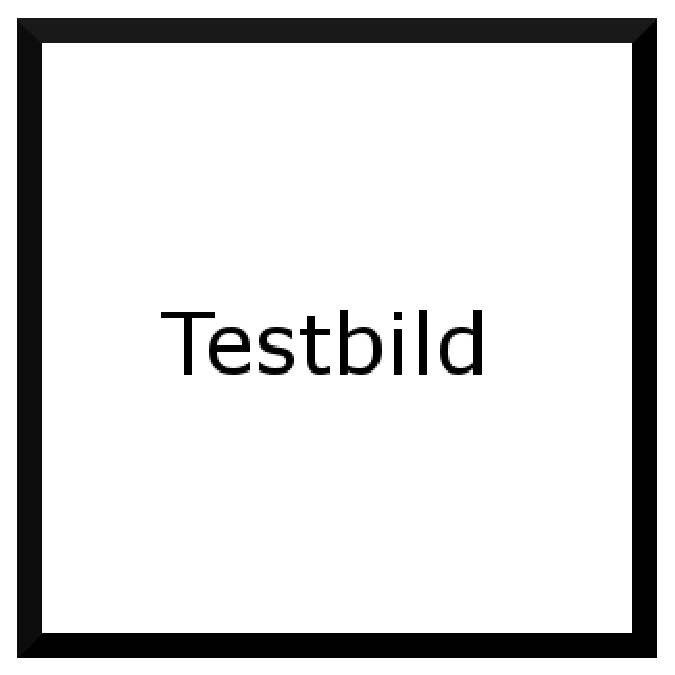
\includegraphics[width=0.33\bildbreite]{bilder/testbild}};
\end{tikzpicture}
\caption[Kurze Abbildungsbeschreibung f"ur das Abbildungsverzeichnis]{Abbildungsbeschreibung f"ur das Testbild\atlbe}
\label{fig:testbild}
\end{figure}

%\begin{figure}[H]\centering
%\includegraphics[scale=0.5]{Bilder/Stromregler.png}
%\caption{Versuchsschaltung Stromregler}
%\label{abb:stromregler}
%\end{figure

\tablename~\ref{tab:testtabelle} zeigt eine Testtabelle. In TexMaker l"a{\ss}t sich relativ schnell und komfortabel eine Tabelle mittels dem eingebauten Tabellen-Assistenten erstellen (zu finden unter \emph{Assistent}$\rightarrow$\emph{Tabellen-Assistent}).

\begin{table}[H]
\caption[Kurze Bennennung der Tabelle mit den technischen Daten f"ur das Tabellenverzeichnis]{Technische Daten\atlbe}
\centering
\begin{tabular}{cc}
\toprule
\multicolumn{2}{c}{\textbf{Testwerte}}\\
\midrule
Kraft & $\SI{1}{kN}$\\
L"ange & $\SI{1}{m}$\\
\bottomrule
\end{tabular}
\label{tab:testtabelle}
\end{table}

Es kann auch eine Schaltung \figurename~\ref{fig:schaltung} in Latex gezeichnet werden.

\begin{figure}[H]
\centering
\begin{circuitikz}[scale=1]\draw
 (0,8) -- (2,8)
 (0,10) node [left] {$U_{IN}$} to [switch, l=$S_1$, o-*] (2,10)
 to [L, l=$L$, *-o] (4,10) to [short, *-o] (5,10) node [right] {$U_{OUT}$}
 (4,10) to [capacitor, l_=$C$, -*] (4,8) node[rground]{}
 (2,8) to [opening switch, l=$S_2$, *-*] (2,10)
 (0,8) node [left] {$GND$} to [short, o-o] (5,8) node [right] {$GND$}
;\end{circuitikz}
\caption[Aufbau buck converter]{Aufbau buck converter\atlbe}
\label{fig:schaltung}
\end{figure}
\ifthenelse{\boolean{english}}{
	\chapter{Test Preparation \& Materials}
}{
	\chapter{Versuchsaufbau \& Materialien}
}
\label{cha:versuchsaufbau}

In \cite{meh10} sind viele interessante Informationen enthalten.

Es kann auch auf \cite{laser2016} verwiesen werden.

In \figurename~\ref{fig:diagramm_beispiel} ist eine Beispielkurve aufgetragen.


\begin{figure}[H]
\centering
\begin{tikzpicture}

\begin{axis}[
%scaled x ticks={base 10:3},
%scaled y ticks={base 10:-3},
width=0.9\diagbreite,
height=1.0\diaghoehe,
%
%title = \textbf{Geschwindigkeitsverlauf gemessen an den Messpunkten am Druckbalken},
%
xlabel=$x\,/\,\si{m}$,
ylabel={$f(x)\,/\,\si{m/s}$},
%yticklabel pos=right,
%
xmax = 6,
xmin = -6,
ymax = 50,
ymin = -10,
xtick={-6,-5,...,6},
%ytick={0,-1,-2,-3,-4,-5,-6,-7,-8,-9,-10},
legend style = {
at = {(0.02,0.97)},
anchor=north west,
cells={anchor=west},
},
%
grid = both,
%minor tick num=0,
minor x tick num={1},
minor y tick num={1},
]
	\addplot[only marks,mark=o,samples=20]{x^2 - x +4};
		\addlegendentry{$f(x) = x^2 - x +4$};
\end{axis}
\end{tikzpicture}
\caption[Kurze Bezeichnung des Diagramms f"ur das Abbildungsverzeichnis]{Beispiel eines Diagramms\atlbe}
\label{fig:diagramm_beispiel}
\end{figure}


In \Gl~\ref{eqn:gleichung_beispiel} ist das dynamische Grundgesetz beschrieben. Die \Gl~\ref{eqn:integral1} zeigt den Allgemeine Zusammenhang von Ort, Geschwindigkeit und Beschleunigung. 

\begin{equation}
	F = m \cdot a
\label{eqn:gleichung_beispiel}
\end{equation}
% Eintr"age in das Symbolverzeichnis
%\nmD[F]{$F$}{Kraft}{\si{N}}	% Bereits im Symbolverzeichnis
\nmD[m]{$m$}{Masse}{\si{kg}}
\nmD[a]{$a$}{Beschleunigung}{\si{m/s^2}}

\begin{equation}
	z(t) = \int\limits_0^t v(t)dt = \iint\limits_0^t a(t)dt
\label{eqn:integral1}
\end{equation}
% Eintr"age in das Symbolverzeichnis
\nmD[v]{$v$}{Geschwindigkeit}{\si{m/s}} 
\nmD[t]{$t$}{Zeit}{\si{s}}
\nmD[z]{$z$}{Auslenkung}{\si{m}}

Der Code, um \figurename~\ref{fig:diagramm_beispiel2} zu erstellen soll zeigen, wie externe Daten z.~B. Messdaten in ein Diagramm eingef"ugt werden k"onnen. Das geht sehr komfortabel.


\begin{figure}[H]
\centering
\begin{tikzpicture}
\begin{axis}[
%scaled x ticks={base 10:3},
%scaled y ticks={base 10:-3},
width=0.9\diagbreite,
height=1.0\diaghoehe,
%
%title = \textbf{Geschwindigkeitsverlauf gemessen an den Messpunkten am Druckbalken},
%
xlabel=$x\,/\,\si{s}$,
ylabel={$Messdaten~und~f(x)\,/\,\si{m}$},
%yticklabel pos=right,
%
xmax = 2*pi+0.001,
xmin = 0,
%ymax = 50,
%ymin = -10,
%xtick={-6,-5,...,6},
%ytick={0,-1,-2,-3,-4,-5,-6,-7,-8,-9,-10},
legend style = {
at = {(0.98,0.97)},
anchor=north east,
cells={anchor=west},
},
%
grid = both,
%minor tick num=0,
minor x tick num={1},
minor y tick num={1},
]
% Diagrammdaten
\pgfplotstableread{diagrammdaten/messdaten_beispiel.txt}\DatatableMessdatenBeispiel
	
	\addplot[only marks,mark=o] table[y = y_m] from \DatatableMessdatenBeispiel ;
		\addlegendentry{Messdaten};
		
	\addplot[samples=500,domain=0:2*pi]{sin(deg(x))};
		\addlegendentry{Fitfunktion $f(x) = \mathrm{sin}(x)$};
\end{axis}
\end{tikzpicture}
\caption[Kurze Bezeichnung des zweiten Diagramms f"ur das Abbildungsverzeichnis]{Zweites Beispiel eines Diagramms\atlbe}
\label{fig:diagramm_beispiel2}
\end{figure}


\begin{equation}
\dot{\textbf{x}} =
\begin{bmatrix}
  \dot{a} \\
  \dot{b} \\
  \ddot{c} \\
  \ddot{d} \\
  \end{bmatrix}
  =
\begin{bmatrix} 
  1 & 0 & 0 & 0 \\
  0 & 1 & 0 & 0 \\
  0 & 0 & \frac{1}{2} & \frac{1}{3} \\
  0 & 0 & 0 & 0
  \end{bmatrix}
\begin{bmatrix}
  x \\
  x_{ab} \\
  \dot{x} \\
  \dot{x}_{ab} \\
  \end{bmatrix}
 +
\begin{bmatrix}
  0 \\
  0 \\
  0 \\
  1 \\
  \end{bmatrix}
 \ddot{z}_{ab}
\label{eqn:matrix_beispiel_1}
\end{equation}


\begin{equation}    
\left( \begin{array}{rrr|r}
     1 & \nicefrac{4}{3} & \nicefrac{5}{3} & \nicefrac{22}{3}\\
     0 & -\nicefrac{8}{3} & \nicefrac{2}{3} & -\nicefrac{14}{3}\\
     0 & \nicefrac{2}{3} & \nicefrac{4}{3} & \nicefrac{8}{3}\\
\end{array}\right)
\label{eqn:matrix_beispiel_2}
\end{equation}


Wenn eine Matrix \textbf{A} ben"otigt wird kann sie so aussehen.

%Abschnitt Zentrierung Anfang
{\par\centering
%\begin{equation} %wird nicht verwendet da der Platz nicht ausreicht
$A$ =
$  \begin{bmatrix}
    0 & 0 & 0 & 1 & 0 & 0 & 0 & 0 \\
	0 & 0 & 0 & 0 & 1 & 0 & 0 & 0 \\
	0 & 0 & 0 & 0 & 0 & 1 & 0 & 0 \\
	0 & 0 & 0 & 0 & 0 & 0 & 1 & 0 \\
	0 & 0 & 0 & 0 & 0 & 0 & 0 & 1 \\
	0 & 0 & 0 & \frac{a}{b} & \frac{aa}{b} & 0 & 0 & 0 \\
	\frac{aaa}{b} & \frac{aaaa}{b} & 0 & \frac{aaaaa}{b} & \frac{aaaaaaa}{b} & \frac{abbccccc}{b} & \frac{adddddddd}{b} & 0 \\
	\frac{a}{b} & 0 & 0 & 0 & \frac{a}{b} & \frac{a}{b} & 0 & 0 \\
	\frac{a}{b} & \frac{a}{b} & 0 & \frac{a}{b} & 0 & \frac{a}{b} & \frac{a}{b} \\
	0 & 0 & 0 & 0 & 0 & 0 & 0 & 0
  \end{bmatrix}$
%\label{eqn_hol:state_1} %wird nicht verwendet da der Platz nicht ausreicht
%\end{equation} 		 %wird nicht verwendet da der Platz nicht ausreicht
%Abschnitt Zentrierung Ende
\par}

%Abstand kann händich eingegeben, sollte aber vermieden werden
\vspace*{0.5cm}

\begin{equation}
b = \begin{bmatrix} 0 & 0 & 0 & 0 & 0 & 0 & 0 & 0 & 0 & 1
  \end{bmatrix}^T
\label{eqn:matrix_beispiel_3}
\end{equation}

Matrix \Gl~\ref{eqn:matrix_beispiel_4} ist als small gekennzeichnt und \Gl~\ref{eqn:matrix_beispiel_5} hat die Normale gr"o{\ss}e.

\begin{equation}
  \mbox{\small $\begin{pmatrix}
 	0	&1	&4	&0\\
 	1	&0	&0	&4\\
 	3	&4	&0	&1\\
 	1	&1	&0	&3
  \end{pmatrix}$}
\label{eqn:matrix_beispiel_4}
\end{equation}

\begin{equation}
  \mbox{ $\begin{pmatrix}
 	0	&1	&4	&0\\
 	1	&0	&0	&4\\
 	3	&4	&0	&1\\
 	1	&1	&0	&3
  \end{pmatrix}$}
\label{eqn:matrix_beispiel_5}
\end{equation}

\ifthenelse{\boolean{english}}{
	\chapter{Test Procedure \& methods}
}{
	\chapter{Versuchsdurchf"uhrung \& Methoden}
}
\label{cha:versuchsdurchfuehrung}

\lstlistingname~\ref{lst:listing_beispiel} zeigt ein Beispiel f"ur die Erfassung eines Quellcodes.

\begin{lstlisting}[caption={[Kurzbezeichnung des Listings f"ur das Quellcodeverzeichnis]Beispiel eines Quellcodes\atlbe},label=lst:listing_beispiel,numbers=left,stepnumber=1,breaklines=true,frame=single]
int a = 1;
int b = 2;
int c;

c = a+b;

\end{lstlisting}
\ifthenelse{\boolean{english}}{
	\chapter{Result \& Interpretation}
}{
	\chapter{Ergebnis \& Interpretation}
}
\label{cha:ergebnis}

Text...

% Literaturverzeichnis IEEE-gerecht
\bibliographystyle{IEEEtran}	
\bibliography{Literatur}

\pagenumbering{Roman}
\setcounter{page}{\value{romancount}}

\newpage

% Nomenklatur
\printnomenclature

\newpage

% Anpassung der Abk"urzungen IN DIE PREAMBLE KOPIEREN!!!
%\renewcommand\figurename{\ifthenelse{\boolean{english}}{Fig.}{Abb.}}
%\renewcommand\tablename{\ifthenelse{\boolean{english}}{Tab.}{Tab.}}
%\renewcommand\lstlistingname{\ifthenelse{\boolean{english}}{Lst.}{Lst.}}
%\newcommand\Gl{\ifthenelse{\boolean{english}}{Eq.}{Gl.}}

% "Uberschriften der Verzeichnisse
\ifthenelse{\boolean{english}}{
\renewcommand{\listfigurename}{List of Figures}
\renewcommand{\listtablename}{List of Tables}
\renewcommand{\lstlistlistingname}{List of Source Code}
}
{
\renewcommand{\listfigurename}{Abbildungsverzeichnis}
\renewcommand{\listtablename}{Tabellenverzeichnis}
\renewcommand{\lstlistlistingname}{Quellcodeverzeichnis}
%\renewcommand{\appendixname}{Anh"ange} --> wird nicht benötigt
}

% Abbildungsverzeichnis
\listoffigures
\addcontentsline{toc}{chapter}{\listfigurename} % f"ugt den Eintrag im Inhaltsverzeichnis hinzu

\newpage

% Tabellenverzeichnis
\listoftables
\addcontentsline{toc}{chapter}{\listtablename} % f"ugt den Eintrag im Inhaltsverzeichnis hinzu

\newpage

% Listingsverzeichnis
\lstlistoflistings 
\addcontentsline{toc}{chapter}{\lstlistlistingname} % f"ugt den Eintrag im Inhaltsverzeichnis hinzu

%Appendix Anhänge --> nicht einfügen Schrottet das Abbildungsverzeichniss
%\appendix 
%\addtocontents{toc}{\protect\setcounter{tocdepth}{-1}} 
%\renewcommand*\appendixpagename{Anhang} 
%\renewcommand{\appendixtocname}{Anhang} 

% Anhänge
%\begin{appendix}
	%% Laborbericht
	%\ifthenelse{\boolean{english}}{
	\chapter{Headline Anhang A}
}{
	\chapter{Überschrift Anhang A}
}
\label{cha:anhang_a}


\section{Datenblatt}
\label{sec:datenblatt}

Sensor Datenblatt Laser Abstands-Sensor M10L/100

%\usepackage{pdfpages} muss aktiviert sein

%pfd in die Seite einfügen
\includepdf[pages={1,2}, pagecommand={\thispagestyle{fancy}},width=1.3\textwidth]{anhang/SensorDatenblatt-f.pdf}


%\end{appendix}

\end{document}
